%%%%%%%%%%%%%%%%%%%%%%%%%%%%%%%%%%%%%%%%%%%%%%%%%%%%%%%%%%%%%%%%%%%%%%
%
% Institut für Rechnergestuetzte Automation
% Forschungsgruppe Industrial Software
% Arbeitsgruppe ESSE
% http://security.inso.tuwien.ac.at/
% lva.security@inso.tuwien.ac.at
%
% Version 2014-04-08
% 
%%%%%%%%%%%%%%%%%%%%%%%%%%%%%%%%%%%%%%%%%%%%%%%%%%%%%%%%%%%%%%%%%%%%%%

\documentclass[12pt,a4paper,titlepage,oneside]{scrartcl}
\usepackage{esseProtocol}
\usepackage{dirtree}
\usepackage{pbox}

%%%%%%%%%%%%%%%%%%%%%%%%%%%%%%%%%%%%%%%%%%%%%%%%%%%%%%%%%%%%%%%%%%%%%%
%
% FOR STUDENTS
%
%%%%%%%%%%%%%%%%%%%%%%%%%%%%%%%%%%%%%%%%%%%%%%%%%%%%%%%%%%%%%%%%%%%%%%

% Group number or "0" for Lab0
\newcommand{\gruppe}{13}
% Date
\newcommand{\datum}{2014-05-16}
% valid values: "Lab0", "Lab1" (be sure to use Uppercase for first character)
\newcommand{\lab}{Lab1}

% name of course
\newcommand{\lvaname}{Security for Systems Engineering}
% number of course
\newcommand{\lvanr}{183.637}
% year and term, for example: "SS 2012", "WS 2012", "SS 2013", etc.
\newcommand{\semester}{SS 2014}

% Student data in Lab0 or 1. student of group in Lab1
\newcommand{\studentAName}{Ren\'{e} Czerny}
\renewcommand{\studentAMatrnr}{0825750}
\newcommand{\studentAEmail}{e0825750@student.tuwien.ac.at}

% 2. student of group in Lab1, for Lab0 or if your group has less students, remove these 3 lines
\newcommand{\studentBName}{Zoltan Krekus}
\renewcommand{\studentBMatrnr}{0702077}
\newcommand{\studentBEmail}{e0702077@student.tuwien.ac.at}

% 3. student of group in Lab1, for Lab0 or if your group has less students, remove these 3 lines
\newcommand{\studentCName}{Philipp Muhoray}
\renewcommand{\studentCMatrnr}{0967964}
\newcommand{\studentCEmail}{e0967964@student.tuwien.ac.at}

% 4. student of group in Lab1, for Lab0 or if your group has less students, remove these 3 lines
\newcommand{\studentDName}{Peter Neubauer}
\renewcommand{\studentDMatrnr}{0725263}
\newcommand{\studentDEmail}{e0725263@student.tuwien.ac.at}

%%%%%%%%%%%%%%%%%%%%%%%%%%%%%%%%%%%%%%%%%%%%%%%%%%%%%%%%%%%%%%%%%%%%%%
%
% DO NOT CHANGE THE FOLLOWING PART
%
%%%%%%%%%%%%%%%%%%%%%%%%%%%%%%%%%%%%%%%%%%%%%%%%%%%%%%%%%%%%%%%%%%%%%%

\newcommand{\lang}{en}
\newcommand{\colormode}{color}
\newcommand{\dokumenttyp}{Report \lab}

\begin{document}

\maketitle
\setcounter{section}{0}
\setcounter{tocdepth}{2}
\tableofcontents

%%%%%%%%%%%%%%%%%%%%%%%%%%%%%%%%%%%%%%%%%%%%%%%%%%%%%%%%%%%%%%%%%%%%%%
%
% CONTENT OF DOCUMENT STARTS HERE
%
%%%%%%%%%%%%%%%%%%%%%%%%%%%%%%%%%%%%%%%%%%%%%%%%%%%%%%%%%%%%%%%%%%%%%%

\section{Lab1a}

\subsection{Notes}
\emph{Notes:}
\begin{itemize}
    \item Either use this English version or the German version in \lstinline{protokoll.tex}
    \item Replace all variables below \emph{FOR STUDENTS} in this .tex file
    \item Replace the placeholders for your name and your student id (MatNr)
    \item Delete these hints and example chapters before the final submission
    \item Keep an eye on the required file formats and \emph{file names} for your submission(s)
    \item Execute \lstinline{pdflatex} at least twice, in order to get correct references and page numbers in the pdf document
    \item You may also use the Makefile for this purpose: \lstinline{make en}
\end{itemize}

\subsection{Sub-Section 1}
Lorem ipsum dolor sit amet, consetetur sadipscing elitr, sed diam nonumy eirmod tempor invidunt ut labore et dolore magna aliquyam erat, sed diam voluptua. At vero eos et accusam et justo duo dolores et ea rebum. Stet clita kasd gubergren, no sea takimata sanctus est Lorem ipsum dolor sit amet. Lorem ipsum dolor sit amet, consetetur sadipscing elitr, sed diam nonumy eirmod tempor invidunt ut labore et dolore magna aliquyam erat, sed diam voluptua. At vero eos et accusam et justo duo dolores et ea rebum. Stet clita kasd gubergren, no sea takimata sanctus est Lorem ipsum dolor sit amet.

\subsection{Sub-Section 2}
Lorem ipsum dolor sit amet, consetetur sadipscing elitr, sed diam nonumy eirmod tempor invidunt ut labore et dolore magna aliquyam erat, sed diam voluptua. At vero eos et accusam et justo duo dolores et ea rebum. Stet clita kasd gubergren, no sea takimata sanctus est Lorem ipsum dolor sit amet. Lorem ipsum dolor sit amet, consetetur sadipscing elitr, sed diam nonumy eirmod tempor invidunt ut labore et dolore magna aliquyam erat, sed diam voluptua. At vero eos et accusam et justo duo dolores et ea rebum. Stet clita kasd gubergren, no sea takimata sanctus est Lorem ipsum dolor sit amet.

\section{Lab1b}

\subsection{Host Discovery and Name Resolution}
The first step to explore the network is to find out which hosts can be found in the networks to scan. To find out which network we are in, we can use the command

\begin{lstlisting}[style=simple]
user13:$ /sbin/ifconfig 
\end{lstlisting}

So we discover, that we are in the network \emph{192.168.98.0/24}. This gives us a good hint where to scan, additionally to the exercise description:

\begin{lstlisting}[style=simple]
user13:$ nmap -sn 192.168.0.0/16
user13:$ nmap -sn 172.16.0.0/16
\end{lstlisting}

The results are as follows:

\begin{tabular}{| l | l |}
\hline
192.168.98.1 & omega.local.vienna.essecorp.invalid \\ \hline
192.168.98.10 & alpha.local.vienna.essecorp.invalid \\ \hline
192.168.98.28 & beta.local.vienna.essecorp.invalid \\ \hline
192.168.98.54 & gamma.local.vienna.essecorp.invalid \\ \hline
192.168.98.99 & delta.local.vienna.essecorp.invalid \\ \hline
192.168.98.124 & tomcat.local.vienna.essecorp.invalid \\ \hline
192.168.98.201 & epsilon.local.vienna.essecorp.invalid \\ \hline
192.168.98.202 & zeta.local.vienna.essecorp.invalid \\ \hline
172.16.2.12 & gemini.dmz.vienna.essecorp.invalid \\ \hline
172.16.2.15 & phoenix.dmz.vienna.essecorp.invalid \\ \hline
172.16.2.25 & taurus.dmz.vienna.essecorp.invalid \\ \hline
172.16.2.253 & lyra.dmz.vienna.essecorp.invalid \\ \hline
\end{tabular}

In order to detect the IPv6 addresses of the found domains we use the fact that nslookup also lists IPv6 addresses for given domains, if we set the type to AAAA:

\begin{lstlisting}[style=simple]
user13:$ nslookup 
>set type=AAAA
alpha.local.vienna.essecorp.invalid
...
\end{lstlisting}

Here are the resulting IPv6 addresses:

\begin{tabular}{| l | l |}
\hline
omega.local.vienna.essecorp.invalid & fdcb:c447:e9d2:3553:1001::1 \\ \hline
alpha.local.vienna.essecorp.invalid & fdcb:c447:e9d2:3553:1001::5 \\ \hline
beta.local.vienna.essecorp.invalid & fdcb:c447:e9d2:3553:1001::9 \\ \hline
gamma.local.vienna.essecorp.invalid & fdcb:c447:e9d2:3553:1001::21 \\ \hline
delta.local.vienna.essecorp.invalid & fdcb:c447:e9d2:3553:1001::43 \\ \hline
tomcat.local.vienna.essecorp.invalid & fdcb:c447:e9d2:3553:1001::ab \\ \hline
epsilon.local.vienna.essecorp.invalid & fdcb:c447:e9d2:3553:1001::79 \\ \hline
zeta.local.vienna.essecorp.invalid & fdcb:c447:e9d2:3553:1001::88 \\ \hline
lyra.dmz.vienna.essecorp.invalid & fdcb:c447:e9d2:3553:1002::fd \\ \hline
\end{tabular}

But what about the IPv6 hosts, who are IPv6-only and have therefore not yet been discovered? Unfortunately nmap does not provide the possibility to scan ranges of IPv6 addresses, which is why we have to create our own ping script and let it run for every subnet in the exercise description (\emph{fdcb:c447:e9d2:3553:1000::} to \emph{fdcb:c447:e9d2:3553:100f::}):

\begin{lstlisting}[style=simple]
for i in `seq 1 255`; do i=$(printf "%x" $i); echo "Trying $i..."; ping6 -c 1 -t 1 "fdcb:c447:e9d2:3553:1000:0000:0000:00$i" > /dev/null && echo "Host $i is running"; done
\end{lstlisting}

However, no additional hosts have been found using this method.

\subsection{MAC addresses}

The MAC addresses have been obtained by looking at the ARP table, and at the information about the own network interfaces. The addresses not currently in the ARP table can be forced into it by simply pinging the required host.

\begin{lstlisting}[style=simple]
user13:$ cat /proc/net/arp | grep 192.168
user13:$ /sbin/ifconfig
\end{lstlisting}

The results are the MAC addresses, which reside in the same subnet.

\begin{tabular}{| l | l |}
\hline
192.168.98.1 & 00:1b:d2:0d:84:98 \\ \hline
192.168.98.10 & 00:1b:d2:d1:1f:85 \\ \hline
192.168.98.28 & 00:1b:d2:f0:60:59 \\ \hline
192.168.98.54 & 00:1b:d2:83:b8:41 \\ \hline
192.168.98.99 & 00:1b:d2:a7:8f:d2 \\ \hline
192.168.98.124 & 00:1b:d2:11:3c:dd \\ \hline
192.168.98.201 & 00:1b:d2:38:ae:b9 \\ \hline
192.168.98.202 & 00:1b:d2:85:9c:c4 \\ \hline
\end{tabular}

\subsection{Operating Systems, Ports and Services}

Nmap also has the possibility to guess operating systems and services behind open ports. Sometimes even version numbers. We used the following commands to gain this information. Regarding the operating system, one can also sometimes guess it looking at the services running. Some only run on Unix systems, for example.

\begin{lstlisting}[style=simple]
user13:$ nmap -A 192.168.98.1/24
user13:$ nmap -A 172.16.2.1/24
\end{lstlisting}

\renewcommand{\arraystretch}{2.5}
\begin{tabular}{| l | l |}
\hline
192.168.98.1 & \pbox[c]{\textwidth}{OS: Linux (Debian kind) \\ 22: SSH - OpenSSH 6.0p1} \\ \hline
192.168.98.10 & \pbox[c]{\textwidth}{OS: Unix  \\ 53: DNS - dnsmasq 2.62} \\ \hline
192.168.98.28 & \pbox[c]{\textwidth}{OS: Unix  \\ 25: SMTP - Exim smtpd 4.80 \\ 110: POP3 - Dovecot pop3d \\ 143: IMAP - Dovecot imapd} \\ \hline
192.168.98.54 & \pbox[c]{\textwidth}{ OS:  \\ 1080: SOCKS - socks5}  \\ \hline
192.168.98.99 & \pbox[c]{\textwidth}{OS: Unix  \\ 631: IPP - CUPS 1.5}  \\ \hline
192.168.98.124 & \pbox[c]{\textwidth}{OS: Linux \\ 8080: HTTP - Apache Tomcat JSP engine 1.1}  \\ \hline
192.168.98.201 & \pbox[c]{\textwidth}{OS: Unix \\ 139: netbios-ssn - Samba 3.6.6 \\ 445: microsoft-ds - Samba 3.6.6}  \\ \hline
192.168.98.202 & all ports closed  \\ \hline
172.16.2.12 & \pbox[c]{\textwidth}{OS: Unix  \\ 80: HTTP - lighttpd 1.4.31}  \\ \hline
172.16.2.15 & \pbox[c]{\textwidth}{OS: Unix \\ 21: FTP - vsftpd 2.3.5}  \\ \hline
172.16.2.25 & \pbox[c]{\textwidth}{OS: Unix \\ 25: SMTP - smtpd 4.8}  \\ \hline
172.16.2.253 & \pbox[c]{\textwidth}{OS: Linux \\ 22: SSH - OpenSSH 6.0p1}  \\ \hline
\end{tabular}

\subsection{Functionality}
The functionality can, of course, only be guessed. However the services provided on the servers give a strong hint to what it might be used for. Also nslookup can be used to guess which computers are probably routers (see Network Topology section).
 
\begin{tabular}{| l | l |}
\hline
192.168.98.1 & router \\ \hline
192.168.98.10 & name server (DNS) \\ \hline
192.168.98.28 & mail server \\ \hline
192.168.98.54 & proxy server \\ \hline
192.168.98.99 & printer server \\ \hline
192.168.98.124 & web application server \\ \hline
192.168.98.201 & file server \\ \hline
192.168.98.202 & unknown \\ \hline
172.16.2.12 & web server \\ \hline
172.16.2.15 & FTP server \\ \hline
172.16.2.25 & mail server (only sending - probably for the tomcat server) \\ \hline
172.16.2.253 & router \\ \hline
\end{tabular}

\subsection{Network Topology}
To discover the network topology, we used trace path, where you can find out which hops a packet needs to pass in order to get to a destination.

\begin{lstlisting}[style=simple]
user13:$ tracepath 172.16.2.12
1:  tomcat.local.vienna.essecorp.invalid                  0.100ms pmtu 1500
1:  omega.local.vienna.essecorp.invalid                  0.721ms 
1:  omega.local.vienna.essecorp.invalid                  0.542ms 
2:  gemini.dmz.vienna.essecorp.invalid                   1.128ms reached
     Resume: pmtu 1500 hops 2 back 63 
\end{lstlisting}

\begin{figure}[h!]
  \centering
  \fbox{
    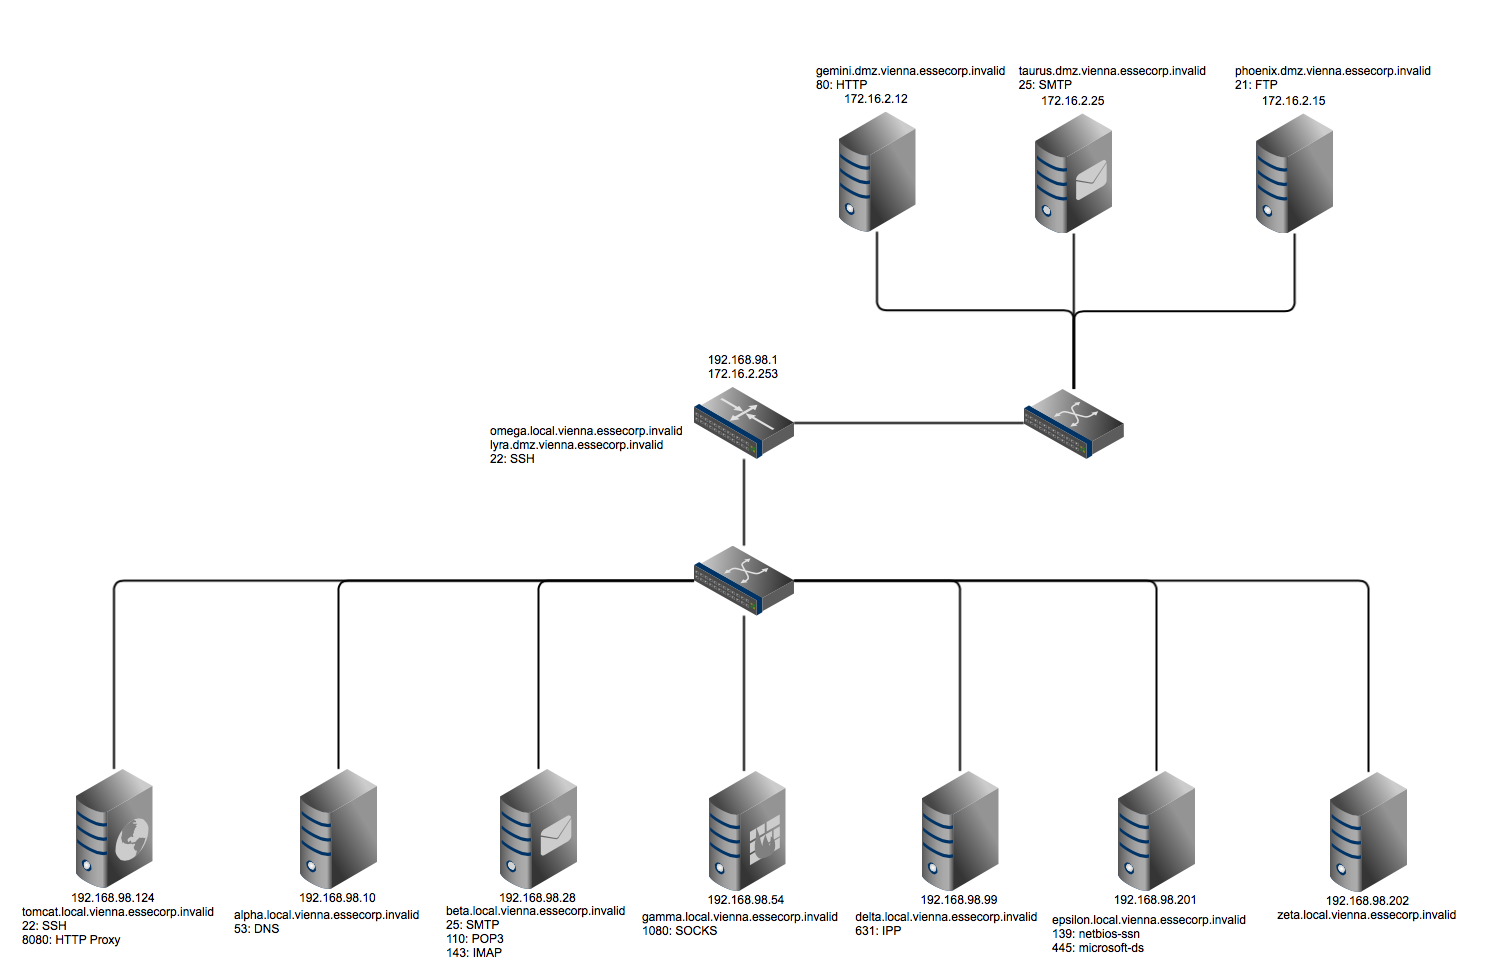
\includegraphics[angle=270,width=0.9\textwidth]{./imgs/network_topology.png}
  }
  \caption{Network Topology}
\end{figure}

\section{Lab1c}

\subsection{A1 - Injection}
This application is a small example of a shell injection vulnerability. Injection in general is a widely distributed vulnerability, which can be used
in various attacks, where one could inject malicious code, get sensitive information, etc.. This example handles a specific version of injection, namely the shell injection. The basis of this vulnerability is, that a user input is forwarded to the system's shell without any validation whatsoever. Attackers can add shell commands to the user input, which will be executed by the program. To counter these attacks, it is necessary to validate the user input, by escaping/removing special characters that are interpreted by the shell, like  \textit{\$, |, \&, <, >, ` and ;}. Even better though, is to completely avoid shell execution from another program, especially if user input is involved.

The example program takes a string as argument and returns it in 1337 speak. It uses the c function
\textit{system(char *string)}, which makes it vulnerable to shell injection (see code line 42 in the vulnerable source code). The fixed program filters
every special character, that could be used in a shell injection and replaces it with an
underscore (see code line 40 and 41 in the fixed source code). Therefore, an attacker is not able to input additional shell commands any more.

The directory structure of the application is as follows:

\dirtree{%
.1 app3. 
.2 exploit. 
.3 Makefile\DTcomment{used to build the example programs}. 
.3 README. 
.2 src-vuln.
.3 1337echo.c\DTcomment{The program vulnerable to shell injection}. 
.2 src-fixed. 
.3 1337echo.c\DTcomment{The program no longer vulnerable to shell injection}. 
}

To compile both the vulnerable and the fixed program, just run

\lstinline{make}

in the \textit{exploit} directory to compile both the vulnerable and the not vulnerable program.

To use the examples after compiling, run 1337echo in the folder \textit{src-vuln} or \textit{src-fixed} (depending on which you want to try):

\lstinline{./1337echo "This is a test!"}

An example exploiting the vulnerability would be (please use with care!):

\lstinline{./1337echo "I will exploit! && rm *"}

An occurrence of a shell injection vulnerability happened in the X.Org X11 server, where remote attackers where allowed to execute commands\footnote{http://www.cvedetails.com/cve/CVE-2011-0465/}. This vulnerability got a CVSS score of 9.3, making it a very delicate one, since it resulted in total information disclosure, total compromise of system integrity and a possibility for total shutdown, while the attacker is not even authenticated.

(\hyperref[code:example1]{see listing~\ref*{code:example1} on page~\pageref*{code:example1}} and \hyperref[code:example2]{see listing~\ref*{code:example2} on page~\pageref*{code:example2}}).

You can include short code snippets or commands directly inline with \lstinline{lstinline block}.

%\lstinputlisting[caption=Example C/C++ file,label=code:example1,style=c]{example.c}

\begin{lstlisting}[caption=Example bash script,label=code:example2,style=simple]
#!/bin/bash
echo "Bash version ${BASH_VERSION}..."
for i in {0..10..2}
  do
     echo "Welcome $i times"
 done

echo "some very very very very very very very very very very very very very very very very very very very very long string"

exit 0;
\end{lstlisting}

\subsection{Images}

Here is an example how to insert an image into this document.
(\hyperref[fig:logo1]{see figure~\ref*{fig:logo1} on page~\pageref*{fig:logo1}}).

\begin{figure}[h!]
  \centering
  \fbox{
    \includegraphics[width=0.4\textwidth]{./imgs/esse-color.png}
  }
  \caption{ESSE Logo}
  \label{fig:logo1}
\end{figure}


%%%%%%%%%%%%%%%%%%%%%%%%%%%%%%%%%%%%%%%%%%%%%%%%%%%%%%%%%%%%%%%%%%%%%%
%
% DO NOT CHANGE THE FOLLOWING PART
%
%%%%%%%%%%%%%%%%%%%%%%%%%%%%%%%%%%%%%%%%%%%%%%%%%%%%%%%%%%%%%%%%%%%%%%

\end{document}


